\documentclass[9pt]{beamer}
% \documentclass[notes, handout, 9pt]{beamer}
% \documentclass[handout, 9pt]{beamer}

\usepackage{import}
\subimport{../}{preamble.tex}
\subimport{../}{beamer-theme.tex}
\usepackage{svg}

% Location for all figures / pictures
\graphicspath{{pictures/}{figures/}}

% % Figures inline
\usepackage{tikz}
\usetikzlibrary{arrows,positioning}

%--------------------------------------------------
% Presentation Information
%--------------------------------------------------
\title[Continuous Optimization]{Dual Spaces, Separation Theorems and Farkas' Lemma}
\author[]{\textbf{Bart Van Parys}}
\date[]{Fall 2026}
%--------------------------------------------------

\begin{document}

\begin{frame}  

  \maketitle

  \vspace{-2em}
  
    \begin{center}
    \begin{tabular}{lll}
      Instructor : & \textbf{Bart Van Parys} & \textbf{(\href{mailto:mastermath@vanparys.xyz}{mastermath@vanparys.xyz})}
    \end{tabular}
  \end{center}
  
\end{frame}

\begin{frame}{Verify Existence of a Solution ?}

  \begin{minipage}{0.5\textwidth}
    Suppose we have the \emph{polyhedral} set
    \[
      C = \set{x\in\Re^n_+} {a_i\tpose x = b_i, \quad i \in [1, \dots, k]}
    \]
    \textbf{Example : $C=\{\rm{system~failure~events}\}$}
  \end{minipage}%
  \hfill
  \begin{minipage}{0.5\textwidth}
    \centering
    \includegraphics[height=3.5cm]{polyhedron/polyhedron.pdf}
  \end{minipage}

  \vfill

  \textbf{How to show that $C \neq \emptyset$?}
  \begin{itemize}
  \item Any element $\bar x \in C$ serves as a \emph{certificate}
  \end{itemize}
  
  
  \vfill

  \textbf{How to show that $C = \emptyset$?}
  \begin{itemize}
  \item Certifying nonexistence seems hard \dots
  \item<2-> Solution at the end of this lecture!
  \end{itemize}

  
\end{frame}


\section{Dual Space}

\begin{frame}{Dual Space}

  Consider a \emph{primal} vector space $E$. Function $f:E\to\Re$
  \begin{itemize}
  \item \emph{Linear} if $f(a x+ by) = a f(x) + b f(y)$ for all $a, b \in \Re$ and $x, y \in E$
  \item \gray{Continuous if $x_i\to\bar x \implies f(x_i)\to f(\bar x)$}
  \end{itemize}
  \vfill

  \begin{minipage}{0.5\textwidth}
    \begin{center}
      \begin{tikzpicture}

        % \draw[draw=blue, thick] plot[id=ex1,domain=-2:2,samples=1000] function {0.4*x};
        \node[draw=blue, fill=blue, inner sep=1] at (-0.4, 1) {};

        % \draw[draw=orange, thick] plot[id=ex1,domain=-2:2,samples=1000] function {-0.7*x};
        \node[draw=orange, fill=orange, inner sep=1] at (-0.35, -0.5) {};

        % \draw[draw=red, thick] plot[id=ex1,domain=-2:2,samples=1000] function {1*x};
        \node[draw=red, fill=red, inner sep=1] at (0.7, -0.7) {};
        
        \draw[->] (-2, 0) -- (2, 0);
        \node[right] at (0.7, 1.8) {$\Re^n$};
        % \node[above] at (-4, 3) {$\Re_+$};
        \draw[->] (0, -2) -- (0, 2);
      \end{tikzpicture}
    \end{center}
  \end{minipage}%
  \hfill
  \begin{minipage}{0.5\textwidth}
    \begin{center}
      \begin{tikzpicture}
        \draw[draw=blue, thick] plot[id=ex1,domain=-2:2,samples=1000] function {0.4*x};

        \draw[draw=orange, thick] plot[id=ex1,domain=-2:2,samples=1000] function {-0.7*x};

        \draw[draw=red, thick] plot[id=ex1,domain=-2:2,samples=1000] function {1*x};
        
        \draw[->] (-2, 0) -- (2, 0);
        \node[right] at (0.7, 1.8) {$\Re^n$};
        % \node[above] at (-4, 3) {$\Re_+$};
        \draw[->] (0, -2) -- (0, 2);
      \end{tikzpicture}
    \end{center}
  \end{minipage}
  
  \vfill

  The set
  \(
    E^\star \defn \set{f:E\to\Re}{f~{\rm{linear\gray{~and~continuous}}}}
  \)
  is a vector space. This vector space is denoted the \emph{dual} vector space of $E$.
\end{frame}

\begin{frame}{Inner Product Space}

  Let $E$ be a vector space equipped with an inner product $\iprod{\cdot}{\cdot}$.

  \vspace{1em}

  \uncover<2->{
  \emph{Inner Product :}  Function $\iprod{\cdot}{\cdot}:E\times E\to\Re$ that satisfies
  \begin{enumerate}
  \item Symmetry: $\iprod{x}{y} = \iprod{y}{x}$
  \item Linearity: $\iprod{a x_1+b x_2}{y} = a \iprod{x_1}{y}+b \iprod{x_2}{y}$
  \item Discrimination: $\iprod{x}{x}\geq 0$, $\iprod{x}{x}=0\implies x=0$
  \end{enumerate}
  }
  \vfill

  \textbf{Examples :}
  \begin{itemize}
  \item The space of vectors in $\Re^n$ with inner product $\iprod{x}{y}=x\tpose y$
  \item The space of $m\times n$ matrices with the inner product $$\iprod{X}{Y} = \tr({X\tpose Y}) =  \sum_{i=1}^m \sum_{j=1}^n X_{ij} Y_{ij}$$
  \end{itemize}

\end{frame}


\begin{frame}{Riesz Representation Theorem}

  \begin{minipage}{0.4\textwidth}
    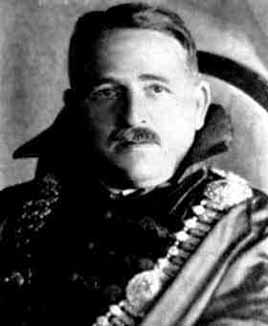
\includegraphics[height=2.5cm]{Riesz.jpeg}

    (Riesz)
  \end{minipage}

  \vfill
  
  \textbf{Theorem (Riesz):} Let $E$ be a finite-dimensional inner product space and $E^\star$ its associated dual space. Let $f\in E^\star$, then there exists a unique $a\in E$ such that
  \[
    f(x) = \iprod{a}{x} \quad \forall x \in E.
  \]

  \vfill

  \uncover<2->{
    \textbf{Moral:} We can represent $E^\star$ as elements from $E$ via an inner product.
    }
\end{frame}

\section{Separation Theorems}

\begin{frame}{Separation Theorems}

  \textbf{General Idea :}
  Let $C, D\subseteq E$ nonempty convex sets such that $\relint(C) \cap \relint(D) = \emptyset$.

  \vfill
  
  \begin{tcolorbox}
    Does there exist a \emph{hyperplane}
    \(
      H\defn  \set{x\in E}{\iprod{a}{x}=b},~ a\neq 0
    \)
    \emph{separating} $C$ from $D$?
  \end{tcolorbox}
  That is, letting $H^{-} \defn \set{x\in E}{\iprod{a}{x}\leq b}$, $H^+\defn \set{x\in E}{\iprod{a}{x}\geq b}$, then $C\subseteq H^-$ and $D\subseteq H^+$.

  \vfill

  \begin{center}
    \includegraphics[height=3cm]{separating-hyperplane/separating-hyperplane.pdf}
  \end{center}

\end{frame}

\begin{frame}{Types of Separation}

  A separation is called
  \begin{itemize}
  \item \emph{proper} if $H \nsupseteq C \cup D$. \emph{Counter-example : }

    \begin{center}
      \includegraphics[height=1cm]{separating-hyperplane/counter-example-proper.pdf}
    \end{center}
  \item<2-> \emph{strict} if $C\subseteq \interior H^{-}$, $D \subseteq \interior H^+$. \emph{Counter-example : }

    \begin{center}
      \includegraphics[height=1.5cm]{separating-hyperplane/counter-example-strict.pdf}
    \end{center}
  \item<3-> \emph{strong} if $C+B(0, \epsilon) \subseteq \interior (H^-)$ and $D+B(0, \epsilon) \subseteq \interior (H^+)$ for some $\epsilon>0$. \emph{Counter-example : }

    \begin{center}
      \includegraphics[height=2.25cm]{separating-hyperplane/counter-example-strong.pdf}
    \end{center}
  \end{itemize}
  
\end{frame}

\begin{frame}{Separation in Terms of Linear Functions}

  \begin{tcolorbox}
    Does there exist a \emph{hyperplane}
    \(
    H\defn  \set{x\in E}{\iprod{a}{x}=b},~ a\neq 0
    \)
    \emph{separating} $C$ from $D$?
  \end{tcolorbox}

  is equivalent according to Riesz to

  \begin{tcolorbox}
    Does there exist a \emph{linear function} $f$ and a number $\alpha$ such that 
    $f(x) \leq \alpha$ for every $x\in C$ and $f(y)\geq \alpha$ for every $y \in D$?    
  \end{tcolorbox}

  \vfill
  \uncover<2->{
  \textbf{Remark :}  
  \begin{itemize}
  \item \emph{Proper} separation : if and only if $f$ is not constantly equal to $\alpha$ on $C\cup D$
  \item \emph{Strict} separation : if and only if equalities are strict
  \item \emph{Strong} separation : if and only if true for all $\alpha \in (\alpha_0 - \epsilon, \alpha_0 + \epsilon)$ for an $\epsilon > 0$
  \end{itemize}
  }
\end{frame}

\begin{frame}{Equivalent Characterizations of Separation}

  \begin{tcolorbox}
    Does there exist a \emph{linear function} $f$ and a number $\alpha$ such that $f(x) \leq \alpha$ for every $x\in C$ and $f(y)\geq \alpha$ for every $y\in D$?    
  \end{tcolorbox}

  \vfill
  \textbf{Remark :}  
  \begin{itemize}
  \item \emph{Proper} separation : if and only if
    \begin{align*}
      \sup \set{f(x)}{x\in C} & \leq \inf \set{f(y)}{y\in D}~\mathrm{and}\\
      \inf \set{f(x)}{x\in C} & < \sup \set{f(y)}{y\in D}
    \end{align*}
    
  \item \emph{Strong} separation : if and only if
    \[
            \sup \set{f(x)}{x\in C} < \inf \set{f(y)}{y\in D}
    \]
  \end{itemize}

\end{frame}

\begin{frame}{Separating Compact Convex Sets}

  \textbf{Theorem :} Let $C, D \subseteq \Re^n$ be nonempty \emph{compact} convex sets and $C\cap D=\emptyset$. There exists a linear function $\hat f$ such that $\sup_{x\in C}\hat f(x) < \inf_{y\in D}\hat f(y)$ (\emph{strong separation}).

  \vfill

  \begin{center}
    \includesvg[height=4.5cm]{separation.svg}
  \end{center}
  
\end{frame}

\begin{frame}{Proof Based on our Classical Results}

  \textbf{Proof:}

  \begin{itemize}
  \item 
    From the \emph{extreme value theorem} we know there exists $d\in D$ and $c \in C$ so that
    \begin{equation}
      \label{eq:minimum_distance}
      0<\norm{d-c}^2_2 = \inf_{x\in C,\,y\in D}\norm{y-x}^2_2.
    \end{equation}
  \item<2->
    As $C\cap D=\emptyset$, we have that $d\neq c$ and hence $a\defn d-c\neq 0$.
  \item<3-> Let $\hat f(x) = \iprod{a}{x}-b = \iprod{d-c}{x-1/2(d+c)}$ with $b = \tfrac{(\norm{d}^2_2-\norm{c}^2_2)}{2}$.
  \item<4-> We claim that $\hat f(x) \leq -\norm{d-c}_2^2/2 < \norm{d-c}_2^2/2 \leq \hat f(y)$ for all $x\in C,~y\in D$.
  \end{itemize}
\end{frame}

\begin{frame}{Proof Based on our Classical Results}

  Let us prove $\hat f(y) \geq \norm{d-c}_2^2/2$ for all $y\in D$. The case $-\norm{d-c}_2^2/2 \geq \hat f(x)$ for all $x\in C$ is completely symmetric.
  \vfill
  \begin{itemize}
  \item<2-> For the sake of contradiction, there exists a $u\in D$ with  $\hat f(u)=\iprod{d-c}{u-d}+\norm{d-c}_2^2/2<\norm{d-c}_2^2/2$.
  \item<3-> Hence, $\iprod{d-c}{u-d}<0$ and $d\neq u$.
  \item<4-> Define $y(t)\defn d+t(u-d)$. We have $y(t)\in D$ for $t\in [0, 1]$ as $D$ is a convex set.
  \item<5-> Let $g(t)\defn \norm{y(t)-c}_2^2$ a continuously differentiable (quadratic) function.
  \item<6-> We have $g'(0)=2 \iprod{d-c}{u-d}<0$. Hence, there exists $0< T\leq 1$ so that for all $t\in [0, T]$ we have $g'(t)<0$. The \emph{mean value theorem} states
    \[
      \norm{d+T(u-d)-c}_2^2 = g(T) = g(0) + g'(t')\, T < \norm{d-c}_2^2
    \]
    for some $t'\in (0, T)$. A contradiction with \eqref{eq:minimum_distance}.
  \end{itemize}

\end{frame}

\begin{frame}{Separation Pitfalls}

  In separation theorems we want to equate $C\cap D=\emptyset$ with (strict/strong) separation. However, we need to be a little cautious even when $C$ and $D$ are convex sets!

  \vfill

  \textbf{Pitfalls:}
  \begin{itemize}
  \item<2-> Strict / Strong separation: may fail when sets are unbounded
    \begin{center}
      \includegraphics[width=0.4\textwidth]{separating-hyperplane/counter-example-strong.pdf}
    \end{center}
  \item<3-> Strict / Strong separation: may fail when sets are open
    \begin{center}
      \includegraphics[width=0.3\textwidth]{separating-hyperplane/counter-example-open.pdf}
    \end{center}
  \end{itemize}
  
\end{frame}

\begin{frame}{Hahn-Banach Extension Theorem}

  \begin{minipage}{0.2\textwidth}
    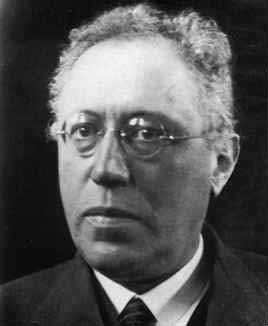
\includegraphics[height=2cm]{Hahn.jpeg}\\
    Hahn
  \end{minipage}%
  \begin{minipage}{0.2\textwidth}
    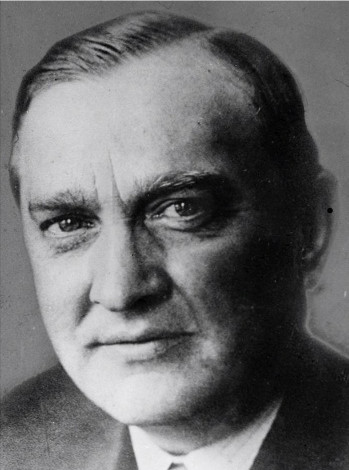
\includegraphics[height=2cm]{Banach.jpeg}\\
    Banach
  \end{minipage}
  \vfill

  \textbf{Elements :}
  \begin{itemize}
  \item $E$ : A vector space
  \item $p:E\to\Re$ : Convex and pos.\ homogeneous function, i.e.\ $p(t x) = t p(x)$ for $t\geq 0$.
  \item $L\subseteq E$ : Linear subspace
  \item $f:L \to \Re$ : Linear function
  \end{itemize}

  Assume
  \(
    f(x) \leq p(x) \quad \forall x\in L .
  \)

  \vfill

  \textbf{Theorem :} It is possible to \emph{extend} $f$ to $E$ while preserving the dominance by $p$. There exists a linear function $\hat f:E \to \Re$ such that $\hat f(x)=f(x)$ for any $x \in L$ and $\hat f(x) \leq p(x)$ for all $x\in E$.
\end{frame}



\begin{frame}{Separating a Point from an Open Convex Set}

  \begin{minipage}{0.5\textwidth}
    \textbf{Theorem :} Let $C \subseteq \Re^n$ nonempty \emph{open} convex set and $D=\{y\}$ where $y\notin C$. There exists a linear function $\hat f$ such that $\hat f(x) < \hat f(y)$ for all $x\in C$.
    \vspace{2em}
  \end{minipage}%
  \hfill
  \begin{minipage}{0.5\textwidth}
    \centering
    \includegraphics[height=3.5cm]{separating-hyperplane/separating-open-set-from-point.pdf}
  \end{minipage}
  \vfill

  \textbf{Proof : }
  \begin{itemize}
  \item<2-> Assume without loss of generality that $0 \in C$, so that $y\neq 0$. Let $p(x) \defn \mu_{C}(x)$ the Minkowski function of $C$. 
  \item<3->  Let $L = \operatorname{span}(y)$ and $f(t y) = t$ for $t\in \Re$.
  \item<4-> We have, $\mu_{C}(y) \geq 1$ because $y\notin C$.  Hence, $\mu_C \geq f$ on subspace $L$.
  \item<5-> Note that $\mu_C(x) < 1$ for any $x$ in $C$ because $C$ is open.
  \item<6-> By Hahn-Banach, there exists a linear function $\hat f$ such that $\hat f(y) = f(y)=1$ and $\hat f(x) \leq \mu_C(x) < 1$ for $x \in C$.
  \end{itemize}

  
\end{frame}

\begin{frame}{Separating a Convex Set from an Open Convex Set}

  \begin{minipage}{0.5\textwidth}
    \textbf{Theorem :} Let $C \subseteq \Re^n$ nonempty \emph{open} convex set and $D$ convex such that $C\cap D = \emptyset$. There exists a linear function $\hat f$ such that $\hat f(x) < \hat f(y)$ for all $x\in C$ and $y\in D$.
    \vspace{2em}
  \end{minipage}%
  \hfill
  \begin{minipage}{0.5\textwidth}
    \centering
    \includegraphics[height=3.5cm]{separating-hyperplane/separating-open-set-from-convex-set.pdf}
  \end{minipage}
  \vfill
  \textbf{Proof [$\star$]: } Let $U = C - D \defn \set{x-y}{x\in C, ~y\in D}$. $C\cap D=\emptyset \implies 0\notin U$. Also, $U$ is open because it is a union of open sets $U=\cup_{y\in D}\set{x-y}{x\in C}$. $U$ is a convex set as it is the Minkowski sum between $C$ and $-D\defn\set{-x}{x\in D}$. We can separate $U$ from the point $\{0\}$, we have
    \[
      \hat f(x-y) < \hat f(0) = 0 ~~\forall x \in C, ~y \in D.
    \]
  Hence, from linearity of $\hat f$ we must have $\hat f(x) < \hat f(y)$ for all $x\in C$ and $y\in D$.
\end{frame}

\begin{frame}{Strong Separation}

  \begin{minipage}{0.5\textwidth}
    \textbf{Theorem :} Let $C \subseteq \Re^n$ convex set with \emph{nonempty} interior and $D=\{y\}$ such that $y\notin \cl(C)$. Then $C$ and $D$ can be strongly separated.
    \vspace{2em}
  \end{minipage}%
  \hfill
  \begin{minipage}{0.5\textwidth}
    \centering
    \includegraphics[height=3.5cm]{separating-hyperplane/separating-convex-set-from-point.pdf}
  \end{minipage}

  \vfill

  \textbf{Proof :} Exactly the same idea. Here, $\mu_C(y) > 1$ and strong separation follows.

  \vfill
  
  \textbf{Corollary :} Let $C\subseteq \Re^n$ convex set with \emph{nonempty interior} and $D$ convex such that $0\notin \cl (C-D)$. Then, $C$ and $D$ can be strongly separated.
  
\end{frame}


\begin{frame}{Fundamental Consequence of Separation Theorems}

  \textbf{Theorem : } Every closed convex set $C \subseteq \Re^n$ is the intersection of the closed half-spaces containing $C$. That is,
  \[
    C = C'\defn\cap_{H~\rm{half-space},\, C\subseteq H} ~H.
  \]

  \vfill
  
  \begin{center}
    \includesvg[height=6cm]{intersection.svg}
  \end{center}

\end{frame}

\begin{frame}{Fundamental Consequence of Separation Theorems -- Proof}

  \textbf{Theorem : } Every closed convex set $C \subseteq \Re^n$ is the intersection of the closed half-spaces containing $C$. That is,
  \[
    C = C'\defn\cap_{H~\rm{half-space},\, C\subseteq H} ~H.
  \]

  \textbf{Proof : }
  \begin{itemize}
  \item<2-> Any arbitrary intersection of convex and closed sets is convex and closed.
  \item<3-> Hence, $C'$ is convex and closed and by construction $C \subseteq C'$.
  \item<4-> We argue that $C'\setminus C = \emptyset$ which implies with $C \subseteq C'$ that $C=C'$.
  \item<5-> For the sake of contradiction, let $x \in C'\setminus C$
  \item<6-> As $x\in\Re^n\setminus C$, which is open, $\exists \epsilon>0$ such that $B(x, \epsilon) \subseteq \Re^n\setminus C$.
  \item<7-> We can separate the open set $B(x, \epsilon)$ from the convex set $C$. That is, $\exists f=\iprod{a}{\cdot}$ linear, $a\neq 0$ with $f(z)<f(y)$ for all $z\in B(x, \epsilon)$, $y\in C$. Hence,
    \[
      t \defn \inf \set{f(z)}{z\in C} \geq \sup \set{f(z)}{z\in B(x, \epsilon)} \geq f(x) + \epsilon \norm{a} > f(x).
    \]
  \item<8-> Consider the half-space $H^+\defn \set{z\in \Re^n}{f(z)\geq t}$, so that $C\subseteq H^+$. $H^+$ is in the collection of half-spaces defining $C'$. However, $x\notin H^+$, a contradiction.
  \end{itemize}
    
\end{frame}

\section{Dual Cone}

\begin{frame}{Dual Cones}

  The \emph{dual cone} of a cone $K$ is the cone $K^\star \defn \set{u}{\iprod{u}{z} \geq 0 ~~\forall z\in K}$.
  
  \vfill

  \textbf{Theorem :} A linear function $f:x\mapsto \iprod{u}{x}$ is nondecreasing, i.e., $x\preceq_{K} y \implies f(x)\leq f(y)$, if and only if
  \(
    u \in K^\star.
  \)

  \vfill
  
  \textbf{Proof [$\star$]:}
  The nondecreasing condition $x\succeq_K y \implies \iprod{u}{x} \geq \iprod{u}{y}$ is equivalent to
  \[
    x - y \in K \implies \iprod{u}{x-y} \geq 0.
  \]
  That is $\iprod{u}{z} \geq 0$ for all $z = x-y \in K$.


\end{frame}

\begin{frame}{Dual Cones for Dummies}

  \begin{enumerate}
    \setlength\itemsep{1em}
  \item  $K^\star$ is closed and convex ($K^\star = \cap_{x\in K} \, \set{u}{\iprod{u}{x}\geq 0}$)

  \item<2->  If $K_1 \subseteq K_2$, then $K_1^\star \supseteq K_2^\star$.

  \item<3-> If $K$ is closed and convex, then $K^{\star\star} =K$.
\end{enumerate}

\end{frame}

\begin{frame}{Proof of $K^{\star\star}=K$}

  \begin{enumerate}
    \setlength\itemsep{1em}
  \item Direction: {$K^{\star \star} \supseteq K$.} Let $\hat x \in K$. As $\iprod{u}{\hat x} = \iprod{\hat x}{u} \geq 0$ for all $u\in K^\star$, we deduce that $\hat x$ in $K^{\star \star}$.

  \item<2-> Direction: $K^{\star \star} \subseteq K$.
    \begin{itemize}
      \setlength\itemsep{0.5em}
    \item<2-> Let $\hat x\notin K$. We prove that $\hat x \notin K^{\star \star}$, i.e., $\exists u \in K^\star$ such that $\iprod{u}{\hat x} < 0$.
    \item<3-> Since $K$ is closed, there exists $\epsilon > 0$ so that $B \defn B(\hat x, \epsilon)$ does not intersect $K$.
    \item<4-> By the separation theorem, we have a linear function $f$ such that $f(x) < f(y)$ for all $x\in B$ and $y \in K$.
    \item<5-> In particular, as $\hat x\in B$ and $0\in K$, we have that $f(\hat x) < 0=f(0)$
    \item<6-> Finally, we have $f(y) \geq 0$ for $y\in K$. Suppose on the contrary that $f(z) < 0$ for a $z\in K$. As $\lambda z\in K$ for all $\lambda >0$, $ f(\lambda z) = \lambda f(z)$ can be taken smaller than $f(\hat x)$, a contradiction.
    \item<7-> We can write $f(x) = \iprod{u}{x}$ and $u$ is what we needed.
    \end{itemize}
         
  \end{enumerate}

\end{frame}


\begin{frame}{Dual Cones Examples}

  \begin{itemize}
    \setlength\itemsep{1em}
  \item $(\Re^m)^\star = \{0\}$
  \item $\{0\}^\star = {\Re^m}$
  \item $(\Re_+^m)^\star = \Re_+^m$ with scalar product $\iprod{x}{y} = x\tpose y$.
  \item<2-> $(S^n_+)^\star = S^n_+$ with the Frobenius scalar product $\iprod{X}{Y} = \tr(X\tpose Y)$.

    \textbf{Proof [$\star$]:} \emph{$(S^n_+)^\star \supseteq S^n_+$.} This follows immediately from $\tr(X\tpose Y)\geq 0$ when $X, Y \in S^n_+$. \emph{$(S^n_+)^\star \subseteq S^n_+$.} Assume that there exists $U \in (S^n_+)^\star$, but $U \notin S^n_+$. Then $U$ has a negative eigenvalue $\lambda_i$ with associated unit eigenvector $u_i$. Denote with $X \defn u_i u_i\tpose$. Then, $X\in S^n_+$ and $\iprod{U}{X} = u_i\tpose U u_i = \lambda_i < 0$, a contradiction.

  \end{itemize}
  
\end{frame}

\section{Farkas' Lemma}

\begin{frame}{Polyhedra}

  \begin{minipage}{0.5\textwidth}
    Suppose we have the \emph{polyhedral} set
    \[
      C = \set{x\in\Re^n_+} {a_i\tpose x = b_i, \quad i \in [1, \dots, k]}
    \]
    \textbf{Example : $C=\{\rm{system~failure~events}\}$}
  \end{minipage}%
  \hfill
  \begin{minipage}{0.5\textwidth}
    \centering
    \includegraphics[height=3.5cm]{polyhedron/polyhedron.pdf}
  \end{minipage}

  \vfill

  \textbf{How to show that $C \neq \emptyset$?}
  \begin{itemize}
  \item Any element $\bar x \in C$ serves as a \emph{certificate}
  \end{itemize}

  \vfill

  \textbf{How to show that $C = \emptyset$?}
  \begin{itemize}
  \item Certifying nonexistence seems hard \dots
  \end{itemize}
  
\end{frame}

\begin{frame}{Separation with Cones}

  \begin{minipage}{0.25\textwidth}
    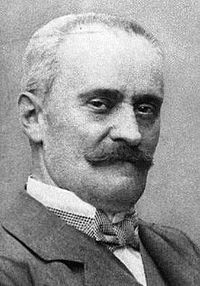
\includegraphics[height=3cm]{Farkas.JPG}\\
    Farkas
  \end{minipage}%
  \hfill
  \begin{minipage}{0.75\textwidth}
    \textbf{Intermediate result :}\\
    Let $A_1, \dots, A_m, b$ in $\Re^n$.
    \begin{equation}
      \label{statement:1}
      \exists t_1, \dots, t_m\in \Re_+ : \quad b = \sum_{i=1}^m t_i A_i
    \end{equation}
    if and only if
    \begin{align}
      \label{statement:2}
      \forall p\in\Re^n ~\st~ & p\tpose A_1\geq 0, \dots, p\tpose A_m \geq 0 : \quad p\tpose b\geq 0 \\
      \uncover<2->{\iff \not \exists p \in \Re^n ~\st~ & p\tpose A_1\geq 0, \dots, p\tpose A_m \geq 0 : \quad p\tpose b<0} \nonumber
    \end{align}
  \end{minipage}

  \vfill

  \uncover<3->{
  \begin{center}
    \includesvg[width=0.4\textwidth]{farkas.svg}
  \end{center}
  }
  
\end{frame}

\begin{frame}{Proof}

  \textbf{Proof:} Let \eqref{statement:1} be the first statement and \eqref{statement:2} the second statement.
  \begin{itemize}
  \item Set $K\defn \cone(\{A_1, \dots, A_m\})$, a convex and closed set (Minkowski--Weyl theorem). Then, $\eqref{statement:1}\iff b\in K$.
  \item Let $p$ such that $p\tpose A_1\geq 0, \dots, p\tpose A_m \geq 0$. By definition then $p\in K^\star$. Hence, $\eqref{statement:2} \iff b\in K^{\star\star}$
  \item<2-> $K=K^{\star\star}$ because $K$ is closed and convex.
  \end{itemize}
  
\end{frame}

\begin{frame}{Farkas' Lemma}

  \textbf{Farkas' Lemma:} Let $A\in\Re^{n\times m}$ and $b\in\Re^n$. Then exactly one of the following systems has a solution
  \begin{enumerate}
  \item $Ax =b$ and $x\succeq_{\Re^m_+} 0$
  \item $A\tpose y \succeq_{\Re^m_+} 0$ and $b\tpose y <0$.
  \end{enumerate}

  \textbf{Proof :} replace $t$ by $x$ and $p$ by $y$ in the intermediate result
\end{frame}

\end{document}
%%% Local Variables:
%%% mode: latex
%%% TeX-master: t
%%% End:
